%% arrowLength=20
%% linkWidth=2
%% input fy=50*node.pos
%% output fx=700
%% output fy=150*node.pos+120
%% MAX_FONT_SIZE=12
\begin{table}[H]
    \begin{center}
        \begin{tabular}{||l c c c||}
            \hline
            & 1        & 2        & 3 \\ [0.5ex]
            \hline
            velikost populacije              & 200      & 250      & 350      \\
            \hline
            največje število vmesnih vozlišč & 15       & 20       & 25       \\
            \hline
            največje število povezav         & 30       & 50       & 75       \\
            \hline
            največje število prečkanj        & 2        & 3        & 4        \\
            \hline
            delež mutiranih potomcev         & 10\%     & 10\%     & 10\%     \\
            \hline
            prispevek kompleksnosti          & -0.00001 & -0.00001 & -0.00001 \\
            \hline
            število generacij                & 300      & 350      & 450      \\
            \hline
        \end{tabular}
    \end{center}
    \caption{Nabori inicializacijskih parametrov poganjanja na množici Wine.}
    \label{tab:param_wine}
\end{table}

\subsection{Prvi nabor}\label{subsec:dodatek-wine-prvi-nabor}
%%"/home/jure/CLionProjects/Neuroevolution/datasets/wine/wine.data" 200 15 30 2 true 0.1 100 true -0.00001 300 ACC
\begin{table}[H]
    \begin{center}
        \begin{tabular}{|| c | c c || c c ||}
            \hline
            \multirow{2}{*}{št. zagona} & \multicolumn{2}{c||}{točnost najboljšega agenta} & \multicolumn{2}{c||}{MKK najboljšega agenta} \\ \cline{2-5}
            & učna   & testna          & učna  & testna                  \\
            \hline
            1         & 80.0\% & 83.0\%          & 0.940 & \textbf{0.943 (96.2\%)} \\
            \hline
            2         & 82.4\% & 83.0\%          & 0.891 & 0.770                   \\
            \hline
            3         & 91.2\% & \textbf{88.7\%} & 0.852 & 0.728                   \\
            \hline
            4         & 95.2\% & 88.7\%          & 0.894 & 0.720                   \\
            \hline
            5         & 90.4\% & 77.4\%          & 0.867 & 0.888                   \\
            \hline
            povprečje & 87.8\% & 84.2\%          & 0.889 & 0.810                   \\
            \hline
            $\sigma$  & 0.057  & 0.042           & 0.030 & 0.090                   \\
            \hline
        \end{tabular}
    \end{center}
    \caption{Rezultat prvega nabora parametrov.}
    \label{tab:wine_result_1}
\end{table}

\begin{table}[H]
    \centering
    \begin{tabular}{||rcccc||}
        \hline
        razred  & Class 1 & Class 2 & Class 3 & vsota \\ \hline
        Class 1 & 17      & 1       & 0       & 18    \\ \hline
        Class 2 & 3       & 18      & 0       & 21    \\ \hline
        Class 3 & 0       & 2       & 12      & 14    \\ \hline
        vsota   & 20      & 21      & 12      & 53    \\ \hline
    \end{tabular}
    \caption{Matrika zmot najbolj točnega agenta prvega nabora.}
    \label{tab:wine_acc_1}
\end{table}

\begin{table}[H]
    \centering
    \begin{tabular}{||rcccc||}
        \hline
        razred  & Class 1 & Class 2 & Class 3 & vsota \\ \hline
        Class 1 & 17      & 1       & 0       & 18    \\ \hline
        Class 2 & 0       & 20      & 1       & 21    \\ \hline
        Class 3 & 0       & 0       & 14      & 14    \\ \hline
        vsota   & 17      & 21      & 15      & 53    \\ \hline
    \end{tabular}
    \caption{Matrika zmot agenta z največjim MKK prvega nabora.}
    \label{tab:wine_mcc_1}
\end{table}

\begin{figure}[H]
    \begin{center}
        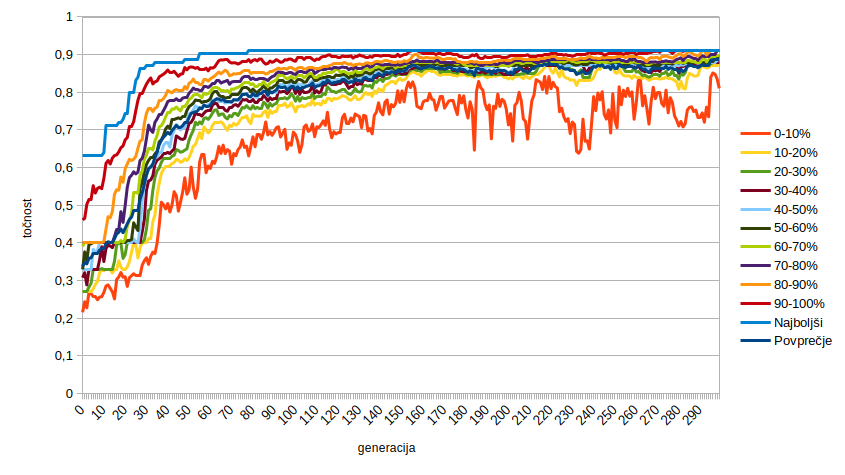
\includegraphics[width=13cm]{wine/1/acc}
    \end{center}
    \caption{Graf točnosti populacije najboljšega agenta prvega nabora skozi generacije.}
    \label{fig:wine_acc_1}
\end{figure}

\begin{figure}[H]
    \begin{center}
        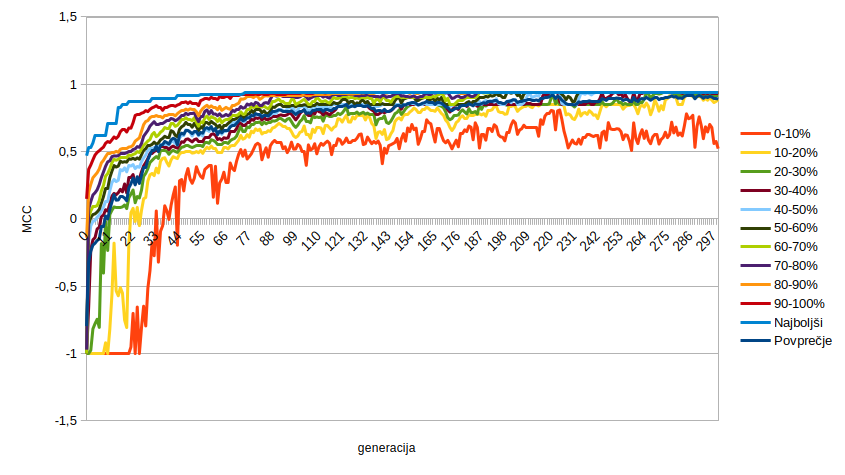
\includegraphics[width=13cm]{wine/1/mcc}
    \end{center}
    \caption{Graf MKK populacije najboljšega agenta prvega nabora skozi generacije.}
    \label{fig:wine_mcc_1}
\end{figure}

\begin{figure}[H]
    \begin{center}
        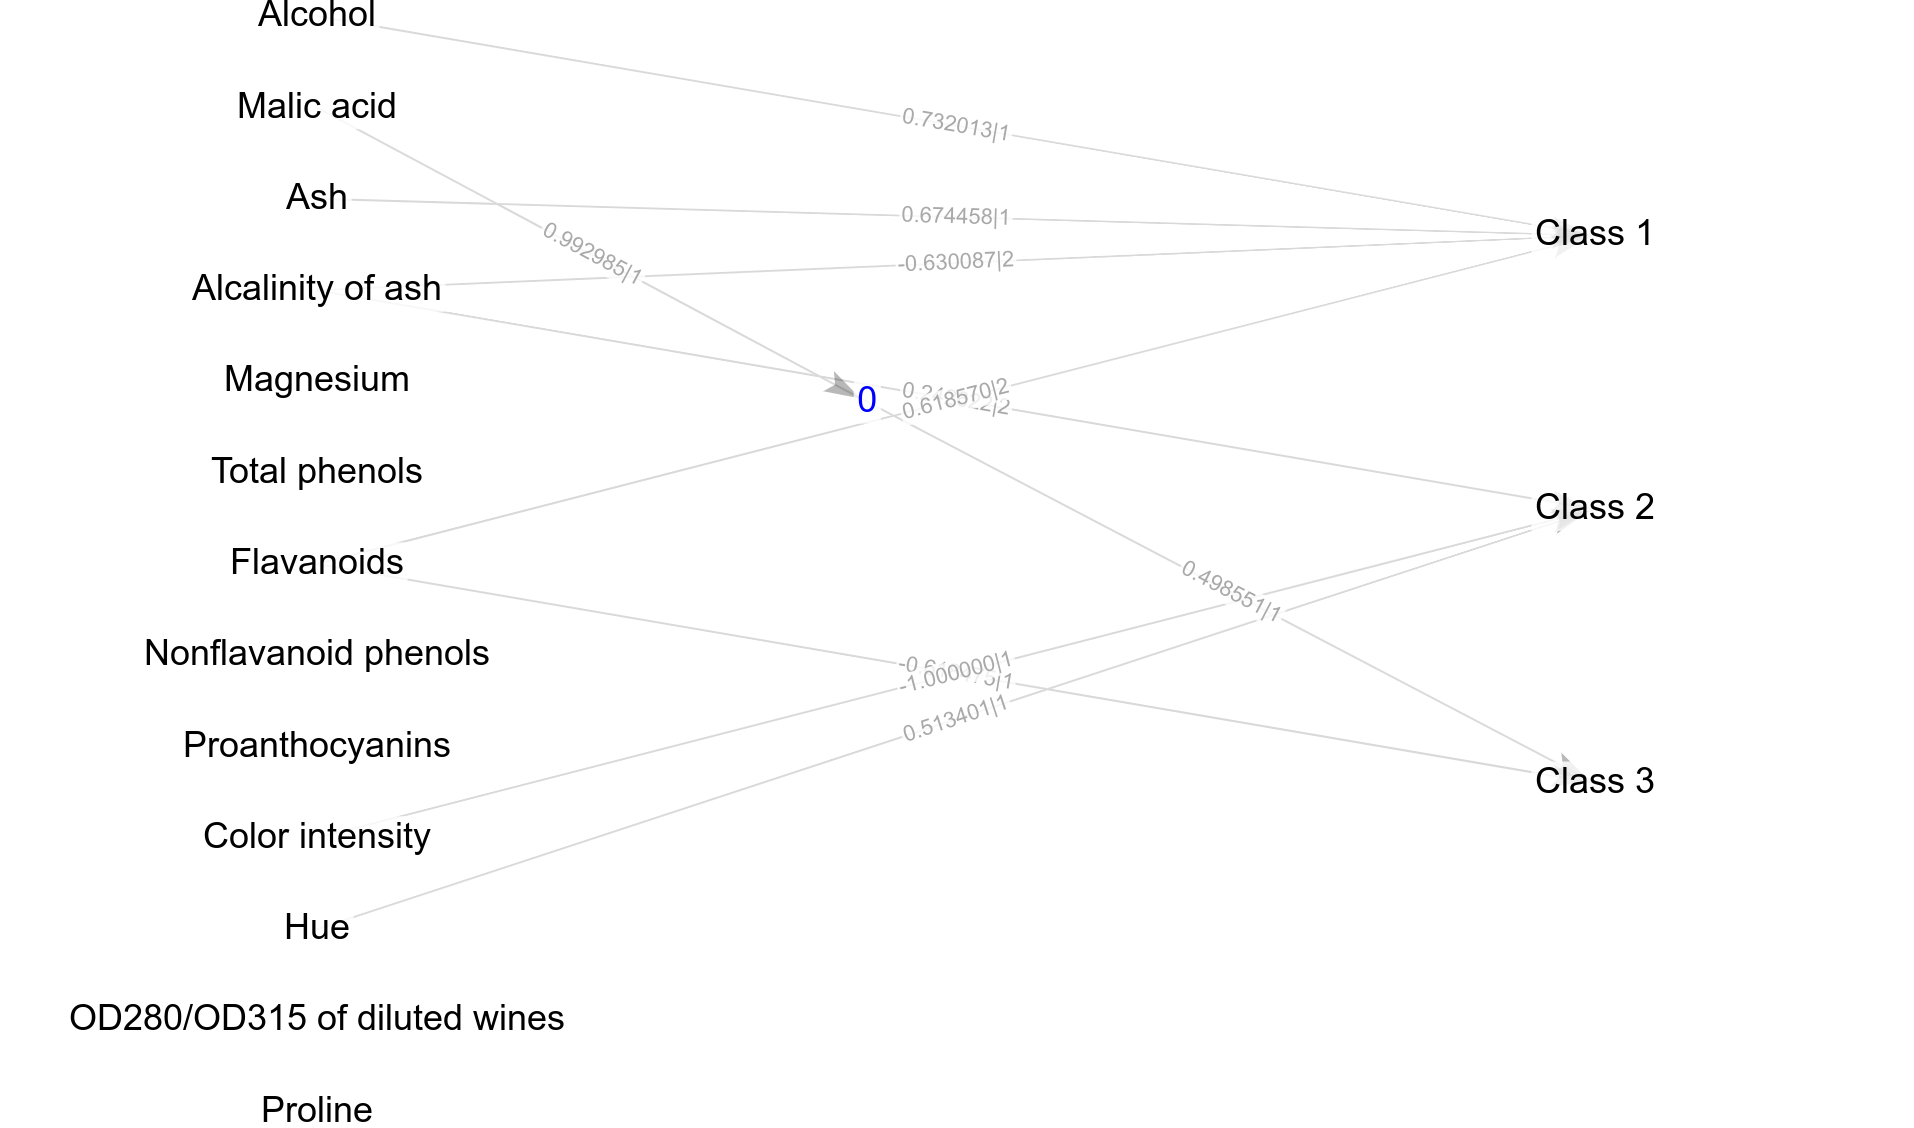
\includegraphics[width=13cm]{wine/1/acc_g}
    \end{center}
    \caption{Vizualizacija najbolj točnega agenta prvega nabora. Vsebuje 1 vmesno vozlišče in 10 povezav.}
    \label{fig:wine_acc_1_g}
\end{figure}

\begin{figure}[H]
    \begin{center}
        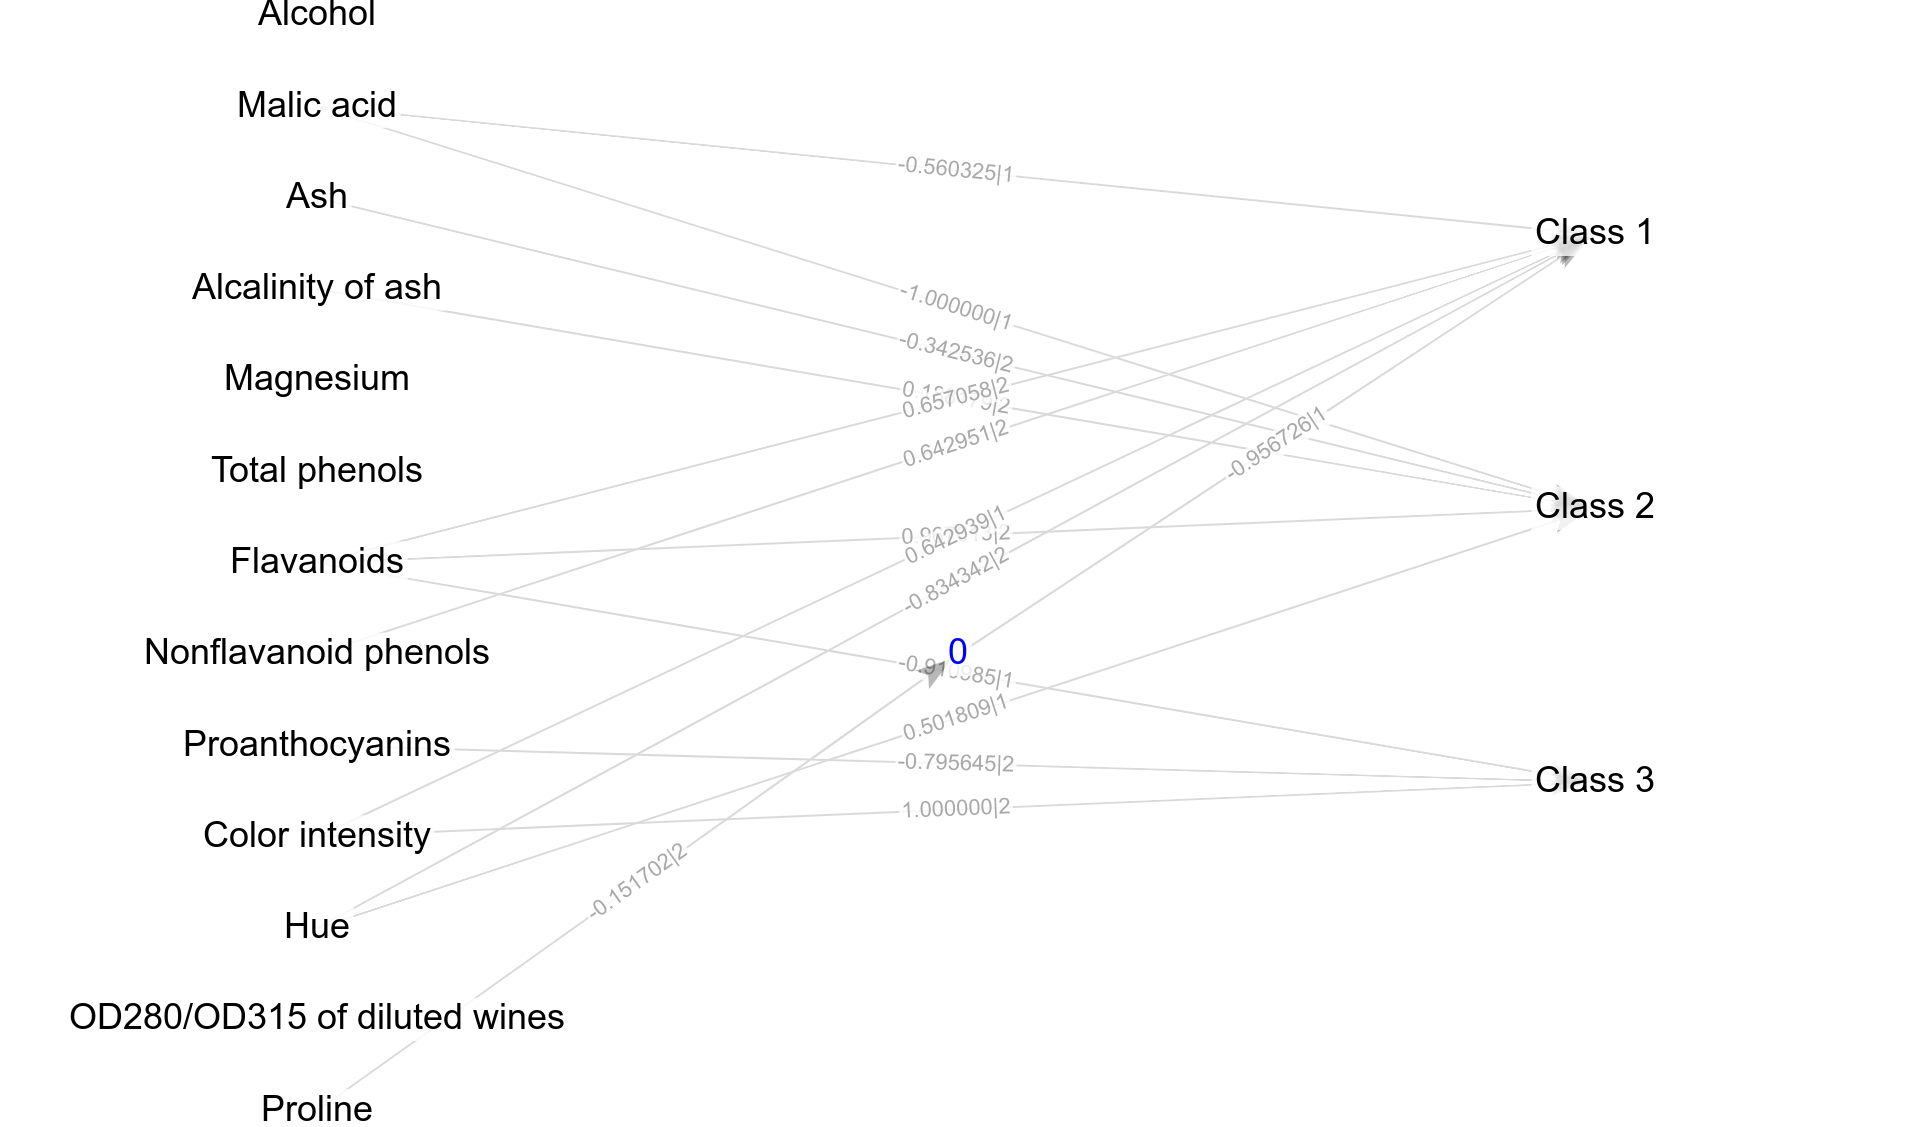
\includegraphics[width=13cm]{wine/1/mcc_g}
    \end{center}
    \caption{Vizualizacija agenta z največjim MKK prvega nabora. Vsebuje 1 vmesno vozlišče in 15 povezav.}
    \label{fig:wine_mcc_1_g}
\end{figure}

\subsection{Drugi nabor}\label{subsec:dodatek-wine-drugi-nabor}
%%"/home/jure/CLionProjects/Neuroevolution/datasets/iris/iris.data" 250 20 50 3 true 0.1 125 true -0.00001 350 ACC
\begin{table}[H]
    \begin{center}
        \begin{tabular}{|| c | c c || c c ||}
            \hline
            \multirow{2}{*}{št. zagona} & \multicolumn{2}{c||}{točnost najboljšega agenta} & \multicolumn{2}{c||}{MKK najboljšega agenta} \\ \cline{2-5}
            & učna   & testna          & učna  & testna                  \\
            \hline
            1        & 95.2\% & \textbf{90.6\%} & 0.906 & \textbf{0.862 (90.6\%)} \\
            \hline
            2        & 72.0\% & 67.9\%          & 0.738 & 0.694                   \\
            \hline
            3        & 80.0\% & 71.7\%          & 0.916 & 0.771                   \\
            \hline
            4        & 93.6\% & 90.6\%          & 0.871 & 0.740                   \\
            \hline
            5        & 91.2\% & 84.9\%          & 0.846 & 0.635                   \\
            \hline
            $\sigma$ & 0.090  & 0.096           & 0.064 & 0.076                   \\
            \hline
        \end{tabular}
    \end{center}
    \caption{Rezultat drugega nabora parametrov.}
    \label{tab:wine_result_2}
\end{table}

\begin{table}[H]
    \centering
    \begin{tabular}{||rcccc||}
        \hline
        razred  & Class 1 & Class 2 & Class 3 & vsota \\ \hline
        Class 1 & 15      & 3       & 0       & 18    \\ \hline
        Class 2 & 0       & 21      & 0       & 21    \\ \hline
        Class 3 & 0       & 2       & 12      & 14    \\ \hline
        vsota   & 15      & 26      & 12      & 53    \\ \hline
    \end{tabular}
    \caption{Matrika zmot najbolj točnega agenta drugega nabora.}
    \label{tab:wine_acc_2}
\end{table}

\begin{table}[H]
    \centering
    \begin{tabular}{||rcccc||}
        \hline
        razred  & Class 1 & Class 2 & Class 3 & vsota \\ \hline
        Class 1 & 14      & 4       & 0       & 18    \\ \hline
        Class 2 & 0       & 20      & 1       & 21    \\ \hline
        Class 3 & 0       & 0       & 14      & 14    \\ \hline
        vsota   & 14      & 24      & 15      & 53    \\ \hline
    \end{tabular}
    \caption{Matrika zmot agenta z največjim MKK drugega nabora.}
    \label{tab:wine_mcc_2}
\end{table}

\begin{figure}[H]
    \begin{center}
        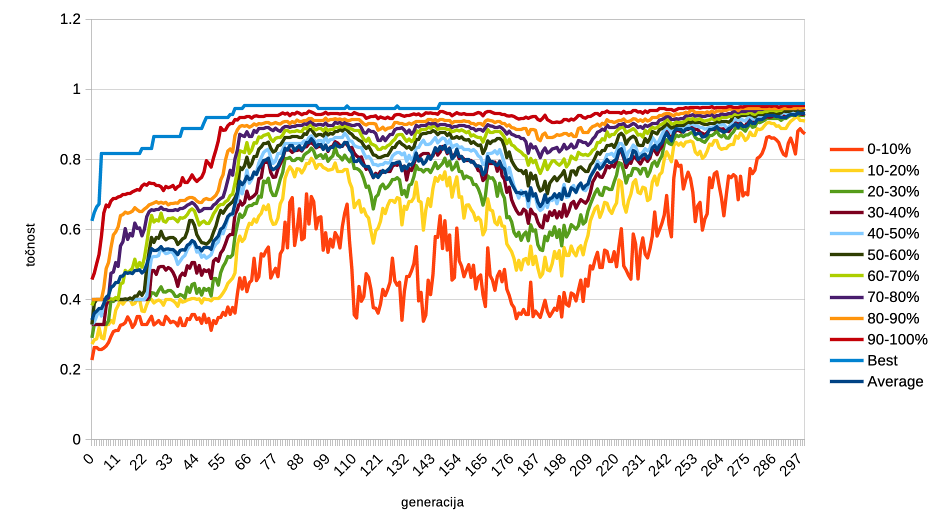
\includegraphics[width=13cm]{wine/2/acc}
    \end{center}
    \caption{Graf točnosti populacije najboljšega agenta drugega nabora skozi generacije.}
    \label{fig:wine_acc_2}
\end{figure}

\begin{figure}[H]
    \begin{center}
        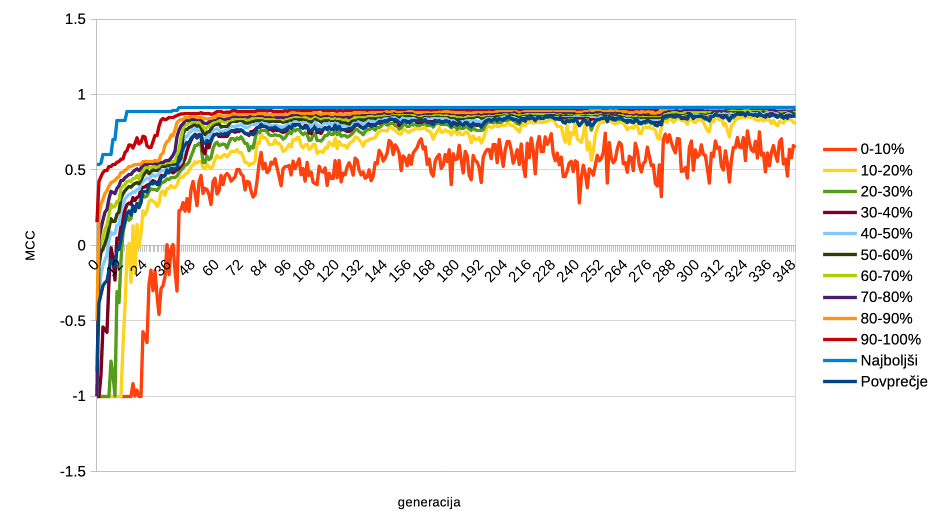
\includegraphics[width=13cm]{wine/2/mcc}
    \end{center}
    \caption{Graf MKK populacije najboljšega agenta drugega nabora skozi generacije.}
    \label{fig:wine_mcc_2}
\end{figure}

\begin{figure}[H]
    \begin{center}
        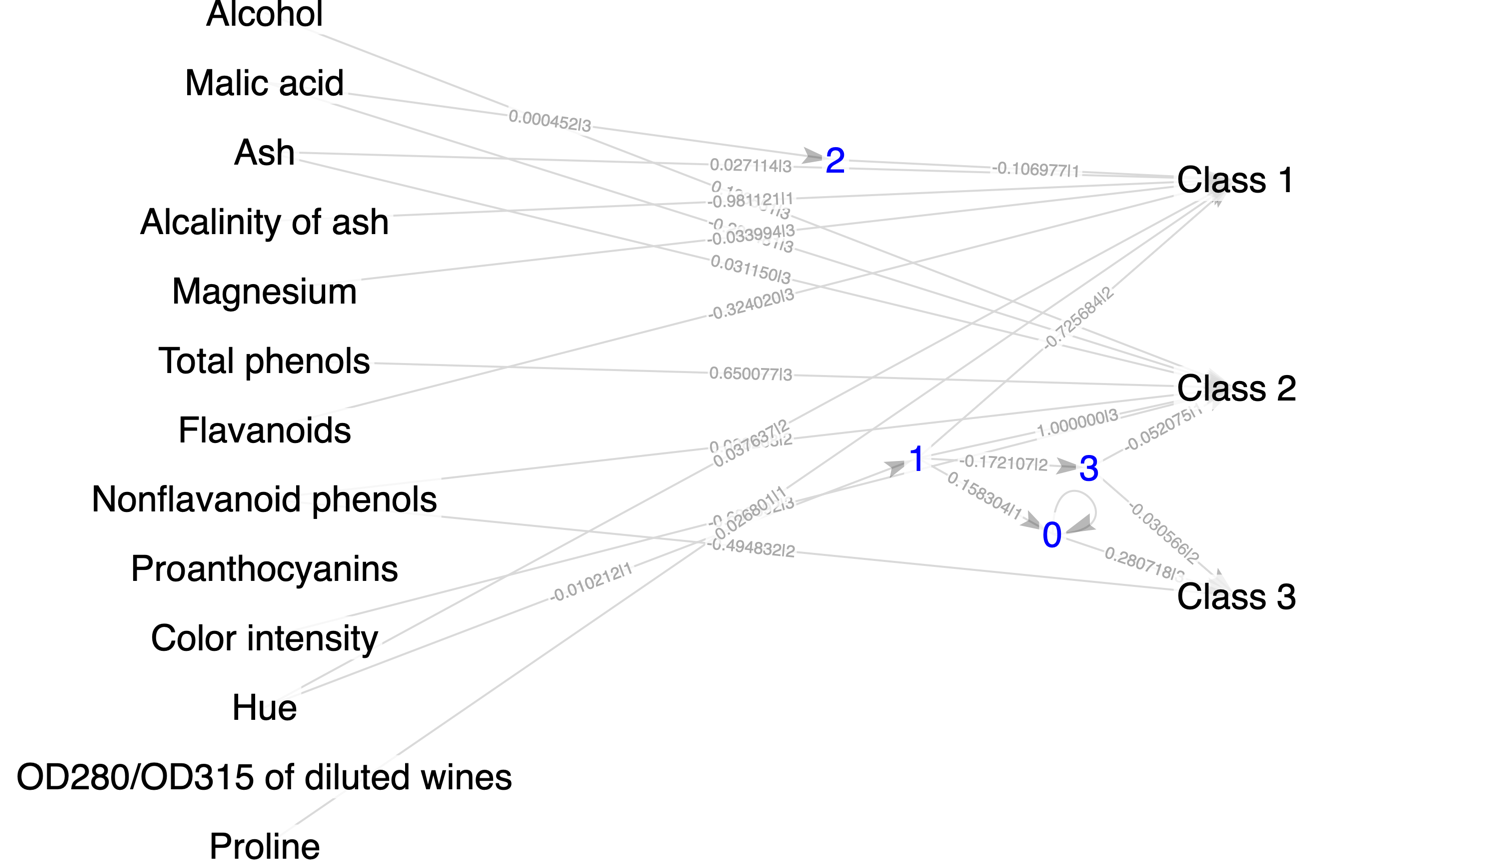
\includegraphics[width=13cm]{wine/2/acc_g}
    \end{center}
    \caption{Vizualizacija najbolj točnega agenta drugega nabora. Vsebuje 1 vmesno vozlišče in 14 povezav.}
    \label{fig:wine_acc_2_g}
\end{figure}

\begin{figure}[H]
    \begin{center}
        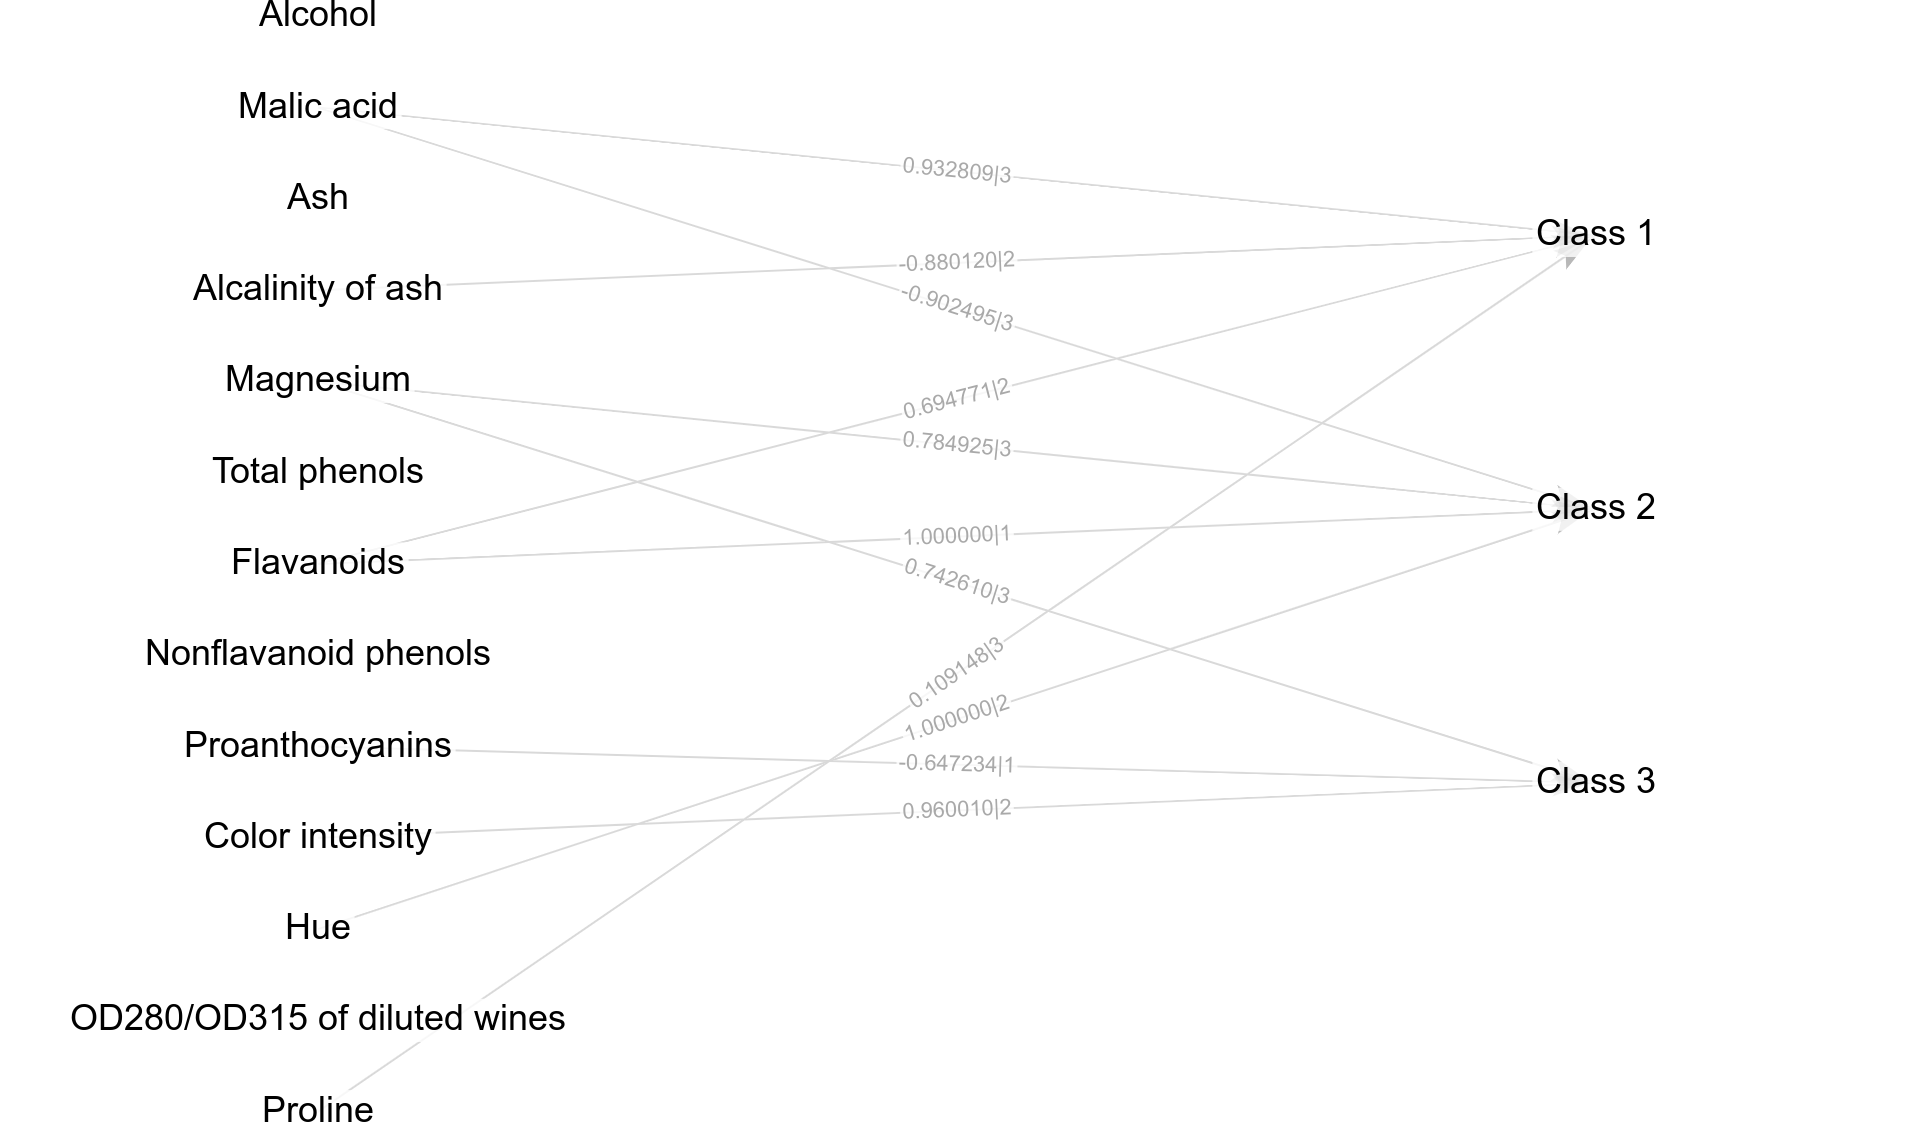
\includegraphics[width=13cm]{wine/2/mcc_g}
    \end{center}
    \caption{Vizualizacija agenta z največjim MKK drugega nabora. Vsebuje 11 povezav.}
    \label{fig:wine_mcc_2_g}
\end{figure}

\subsection{Tretji nabor}\label{subsec:dodatek-wine-tretji-nabor}
%%"/home/jure/CLionProjects/Neuroevolution/datasets/iris/iris.data" 350 25 75 4 true 0.1 175 true -0.00001 450 ACC
\begin{table}[H]
    \begin{center}
        \begin{tabular}{|| c | c c || c c ||}
            \hline
            \multirow{2}{*}{št. zagona} & \multicolumn{2}{c||}{točnost najboljšega agenta} & \multicolumn{2}{c||}{MKK najboljšega agenta} \\ \cline{2-5}
            & učna   & testna          & učna  & testna                  \\
            \hline
            1        & 93.6\% & 90.6\%          & 0.908 & 0.807                   \\
            \hline
            2        & 95.2\% & 90.6\%          & 0.868 & 0.752                   \\
            \hline
            3        & 92.8\% & 86.8\%          & 0.906 & 0.867                   \\
            \hline
            4        & 80.0\% & 77.4\%          & 0.856 & \textbf{0.890 (92.5\%)} \\
            \hline
            5        & 89.6\% & \textbf{92.5\%} & 0.908 & 0.888                   \\
            \hline
            $\sigma$ & 0.054  & 0.054           & 0.023 & 0.054                   \\
            \hline
        \end{tabular}
    \end{center}
    \caption{Rezultat tretjega nabora parametrov.}
    \label{tab:wine_result_3}
\end{table}

\begin{table}[H]
    \centering
    \begin{tabular}{||rcccc||}
        \hline
        razred  & Class 1 & Class 2 & Class 3 & vsota \\ \hline
        Class 1 & 15      & 3       & 0       & 18    \\ \hline
        Class 2 & 0       & 20      & 1       & 21    \\ \hline
        Class 3 & 0       & 0       & 14      & 14    \\ \hline
        vsota   & 15      & 23      & 15      & 53    \\ \hline
    \end{tabular}
    \caption{Matrika zmot najbolj točnega agenta tretjega nabora.}
    \label{tab:wine_acc_3}
\end{table}

\begin{table}[H]
    \centering
    \begin{tabular}{||rcccc||}
        \hline
        razred  & Class 1 & Class 2 & Class 3 & vsota \\ \hline
        Class 1 & 18      & 0       & 0       & 18    \\ \hline
        Class 2 & 2       & 18      & 1       & 21    \\ \hline
        Class 3 & 1       & 0       & 13      & 14    \\ \hline
        vsota   & 21      & 18      & 14      & 53    \\ \hline
    \end{tabular}
    \caption{Matrika zmot agenta z največjim MKK tretjega nabora.}
    \label{tab:wine_mcc_3}
\end{table}

\begin{figure}[H]
    \begin{center}
        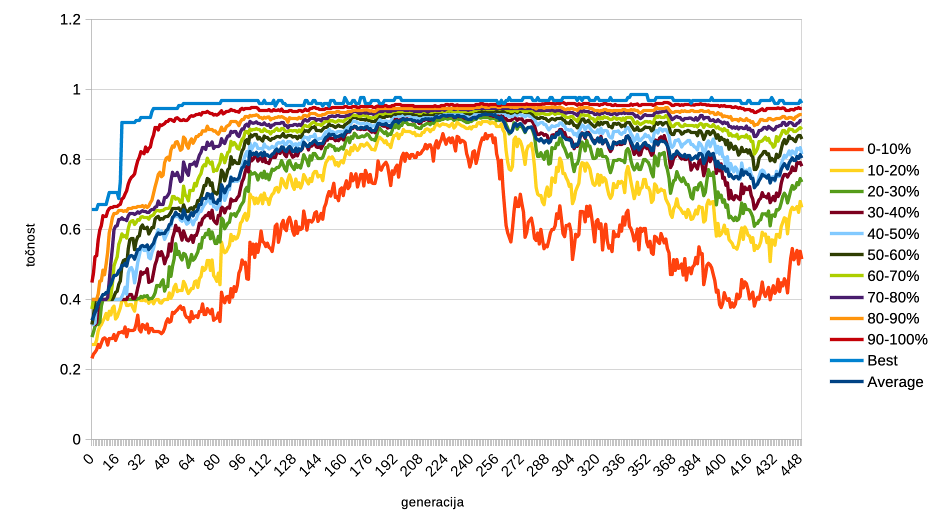
\includegraphics[width=13cm]{wine/3/acc}
    \end{center}
    \caption{Graf točnosti populacije najboljšega agenta tretjega nabora skozi generacije.}
    \label{fig:wine_acc_3}
\end{figure}

\begin{figure}[H]
    \begin{center}
        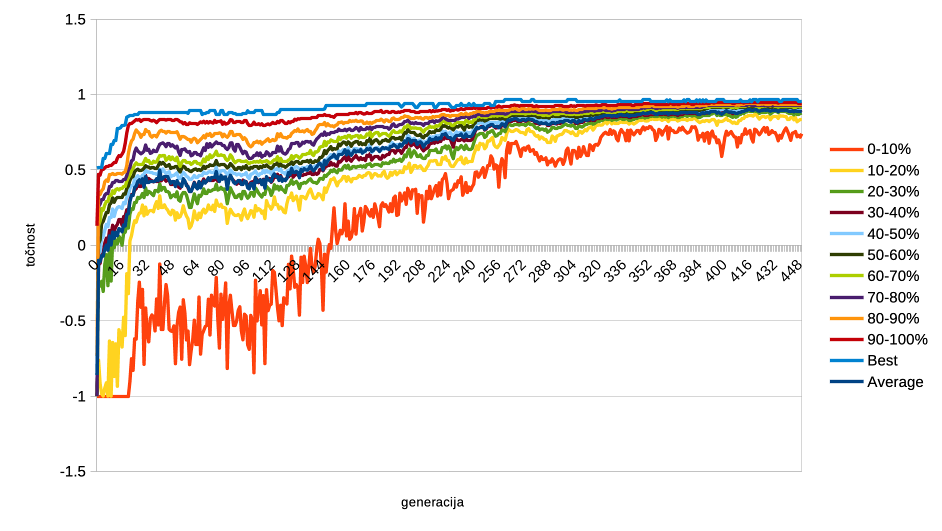
\includegraphics[width=13cm]{wine/3/mcc}
    \end{center}
    \caption{Graf MKK populacije najboljšega agenta tretjega nabora skozi generacije.}
    \label{fig:wine_mcc_3}
\end{figure}

\begin{figure}[H]
    \begin{center}
        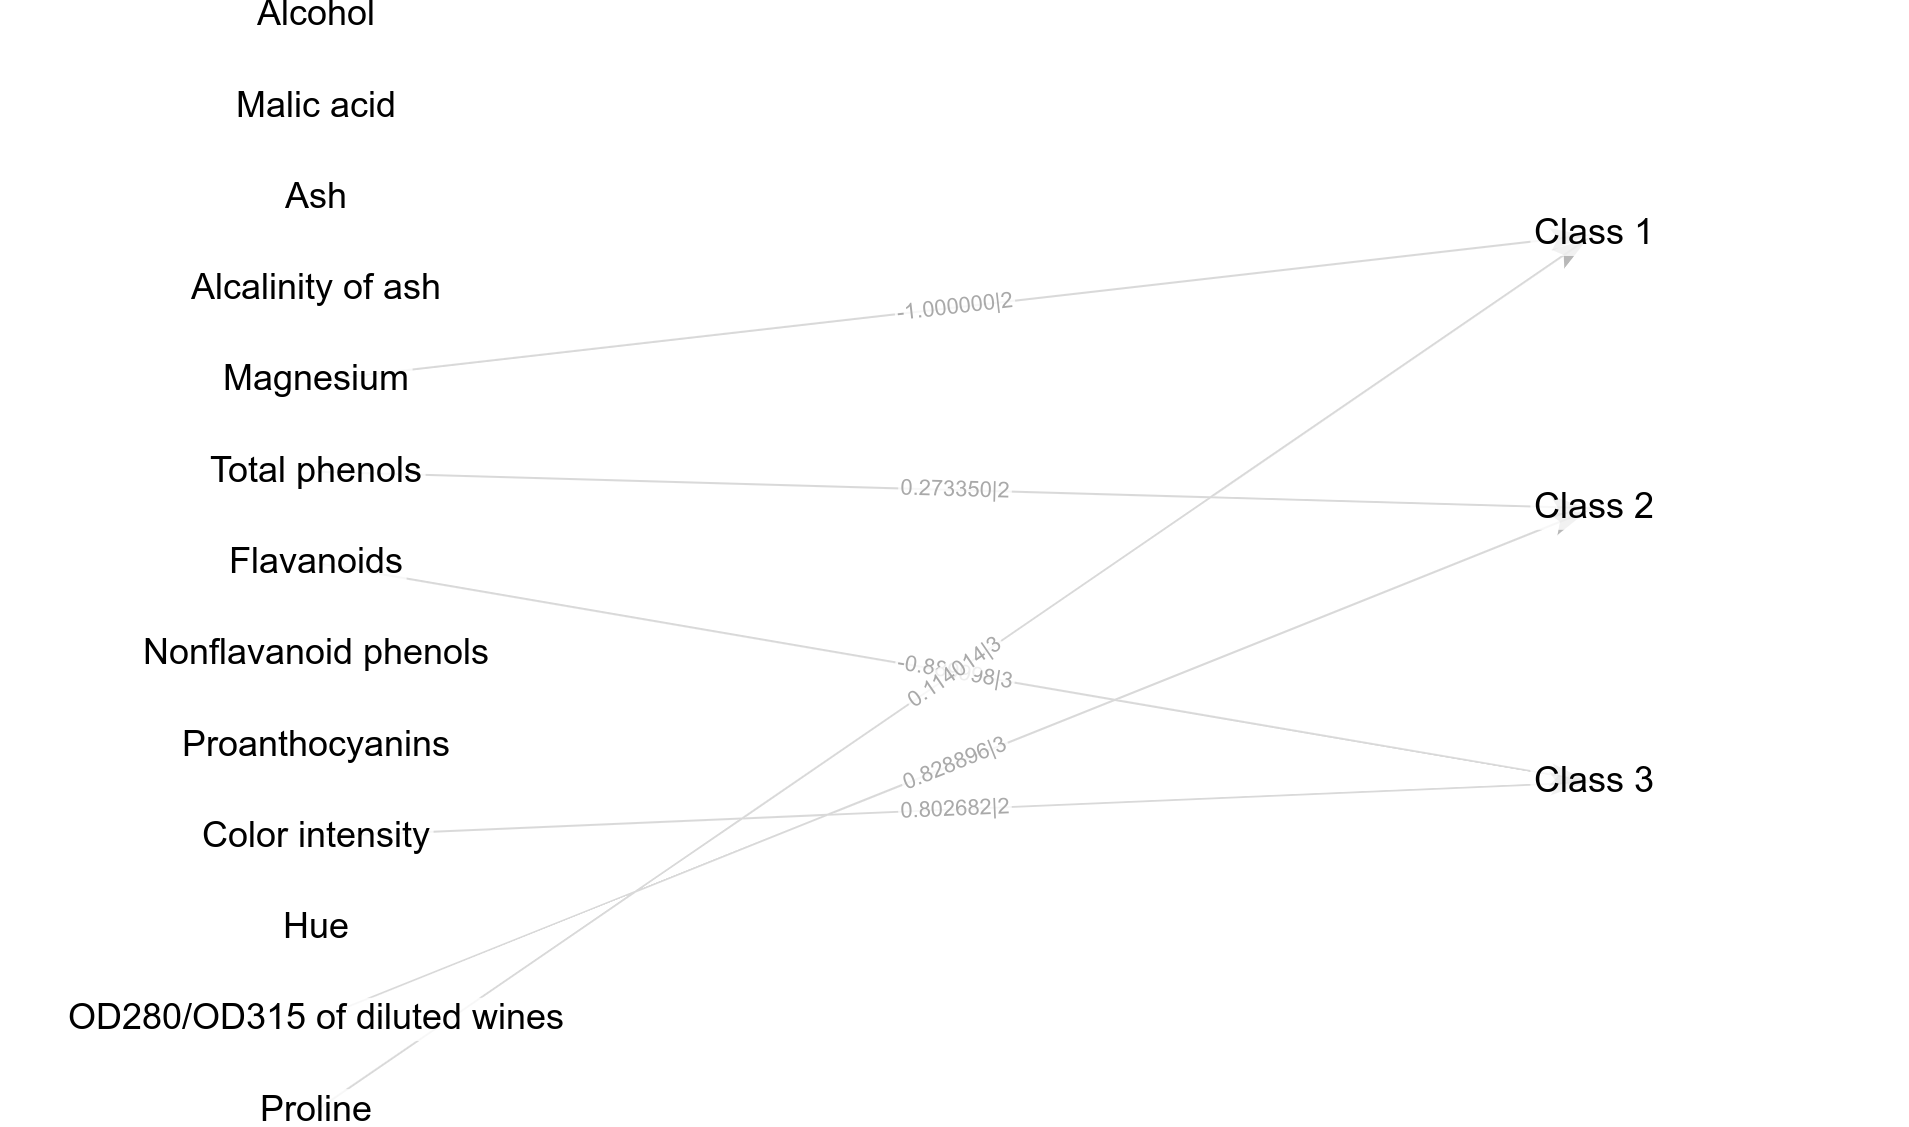
\includegraphics[width=13cm]{wine/3/acc_g}
    \end{center}
    \caption{Vizualizacija najbolj točnega agenta tretjega nabora. Vsebuje 6 povezav.}
    \label{fig:wine_acc_3_g}
\end{figure}

\begin{figure}[H]
    \begin{center}
        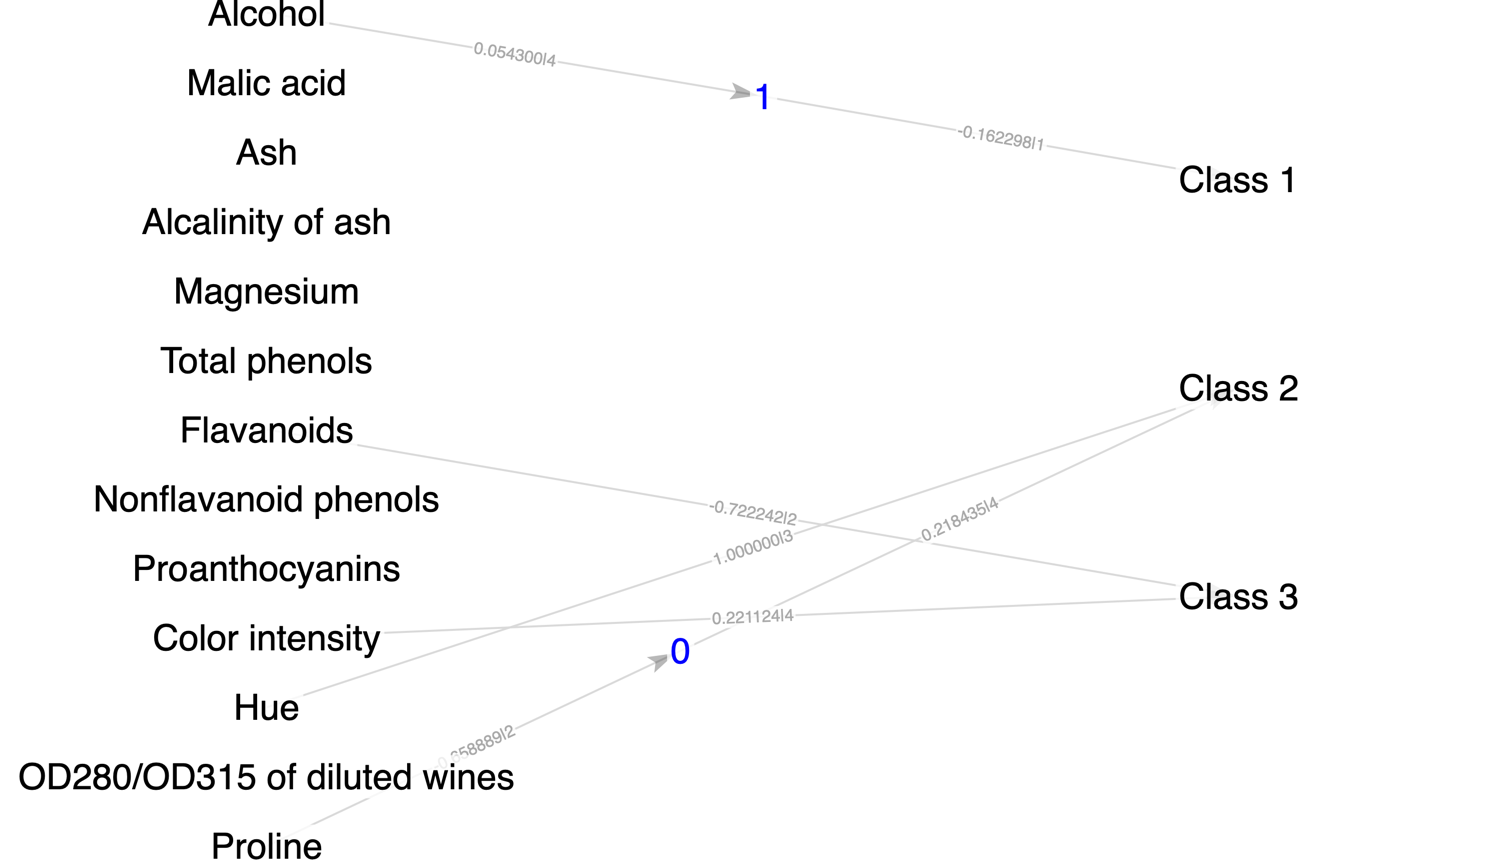
\includegraphics[width=13cm]{wine/3/mcc_g}
    \end{center}
    \caption{Vizualizacija agenta z največjim MKK tretjega nabora. Vsebuje 10 povezav.}
    \label{fig:wine_mcc_3_g}
\end{figure}